\documentclass[openany]{book}  % Openany removes the blank pages between 2 chapters
\usepackage{color}
\usepackage{xcolor}
\usepackage{graphicx}   
\usepackage{graphics}                %  For Inserting List of Figures
\usepackage{index}                      %  For Inserting Index in the document
\usepackage{url,hyperref}               %  For Inserting Index in the document
\usepackage[xindy]{imakeidx}            %  For Inserting Index in Alphabetical order
%\usepackage{float}                      %  For Preventing Table Repositioning
\usepackage{float}                      %  For Preventing Table Repositioning
% \usepackage{geometry}
\usepackage[a4paper,showframe]{geometry} % Change while production

\makeindex                              %  For Inserting Index in the document

\pdfpagewidth 6in
\pdfpageheight 9in


\definecolor{smokeWhite}{HTML}{F5F5F5}
\begin{document}

\begin{titlepage}
    \pagecolor{black}
    \color{white}
    \noindent{\Huge \textbf{JAVA Simplica}}\\
    {\large{$1^{st}$ Edition,}}
    {\Large{Sudipta Kumar Das}}
    \vspace*{\fill}
    \begin{center}
        \tiny{
            \begin{verbatim}
                                                                                                              
                                                                                                                                                                                                                                                          
              
            























                                                                                                                                 
                                                                                                                                 
                                  JJJJJJJJJJJ                    AAA                    VVVVVVVV           VVVVVVVV                    AAA               
                                  J:::::::::J                   A:::A                   V::::::V           V::::::V                   A:::A              
                                  J:::::::::J                  A:::::A                  V::::::V           V::::::V                  A:::::A             
                                  JJ:::::::JJ                 A:::::::A                 V::::::V           V::::::V                 A:::::::A            
                                    J:::::J                  A:::::::::A                 V:::::V           V:::::V                 A:::::::::A           
                                    J:::::J                 A:::::A:::::A                 V:::::V         V:::::V                 A:::::A:::::A          
                                    J:::::J                A:::::A A:::::A                 V:::::V       V:::::V                 A:::::A A:::::A         
                                    J:::::j               A:::::A   A:::::A                 V:::::V     V:::::V                 A:::::A   A:::::A        
                                    J:::::J              A:::::A     A:::::A                 V:::::V   V:::::V                 A:::::A     A:::::A       
                        JJJJJJJ     J:::::J             A:::::AAAAAAAAA:::::A                 V:::::V V:::::V                 A:::::AAAAAAAAA:::::A      
                        J:::::J     J:::::J            A:::::::::::::::::::::A                 V:::::V:::::V                 A:::::::::::::::::::::A     
                        J::::::J   J::::::J           A:::::AAAAAAAAAAAAA:::::A                 V:::::::::V                 A:::::AAAAAAAAAAAAA:::::A    
                        J:::::::JJJ:::::::J          A:::::A             A:::::A                 V:::::::V                 A:::::A             A:::::A   
                         JJ:::::::::::::JJ          A:::::A               A:::::A                 V:::::V                 A:::::A               A:::::A  
                           JJ:::::::::JJ           A:::::A                 A:::::A                 V:::V                 A:::::A                 A:::::A 
                             JJJJJJJJJ            AAAAAAA                   AAAAAAA                 VVV                 AAAAAAA                   AAAAAAA
                                                                                                                                                 
                                                                                                                                                 
                                                                                                                                                 
                                                                                                                                                 
                                                                                                                                                 
                                                                                                                                                 
                                                                                                                                                                                                                                                                                      
                                                                                                                                                                                                                                                                            
                                                                                                                                                                                                                                                                            
                                                        _____   _____   __  __   _____    _        _____    _____            
                                                       / ____| |_   _| |  \/  | |  __ \  | |      |_   _|  / ____|     /\    
                                                      | (___     | |   | \  / | | |__) | | |        | |   | |         /  \   
                                                       \___ \    | |   | |\/| | |  ___/  | |        | |   | |        / /\ \  
                                                       ____) |  _| |_  | |  | | | |      | |____   _| |_  | |____   / ____ \ 
                                                      |_____/  |_____| |_|  |_| |_|      |______| |_____|  \_____| /_/    \_\
                                                                                            
                                                                                                                                                                                                              
                                                                                                                                                              
                                                                                                                                                                                                                                                                     
                                                                                                                                                                                                                                                                            
                                                                                                      
                                                                                                      
        \end{verbatim}
        }
    \end{center}
    \vfill
    \vspace*{\fill}
    {\small{2022, Publisher}}
\end{titlepage}

\vspace*{\fill}

\pagecolor{smokeWhite}
\color{black}
\newpage
\tableofcontents
\newpage
\listoffigures
\newpage
\listoftables
\newpage
\setlength{\evensidemargin}{1.44614pt}           %  Margin Setting
% 
% Part 1
% 
\part{Introduction}
\vspace*{\fill}
JAVA\cite{Ref1} is a Programming language which is used mostly in official softwares because of it's strong security system.
It is a high-level language which uses JVM to convert the high-level code to a machine code.
It is one of the most popular programming languages out there. Released in 1995 and still widely used today.
Java has many applications, including software development, mobile applications, and large systems development.
Knowing Java opens a lot of possibilities for us as a developer.
\vspace*{\fill}

\chapter*{Preface}
JAVA\cite{Ref1} knowledge is vast. People most often have to go through most of the documentations of the JAVA code then they could think of writing something.
Moreover, sometimes people looses their interest in learning JAVA or writing their codes in JAVA. So in that case they just give online posts
and hire outworkers to complete their school/college projects, homeworks and others.
This process's is both insecure and costly. In this book I just tried to teach JAVA in a simple way and by which
people can start doing their school/college projects, homeworks and others by their own, having simple knowledge. Thus, they can learn the vast knowledge slowly and more interesting way.

\addcontentsline{toc}{chapter}{Preface}
% 
% Chapter 1
% 
\chapter{History of JAVA}
Java\cite{Ref1} was originally developed by James Gosling\cite{Ref2}\index{James Gosling} at Sun Microsystems and released in May 1995 as a core component of Sun Microsystems' Java platform.
The original and reference implementation Java compilers\index{Java compilers}, virtual machines\index{virtual machines}, and class libraries\index{class libraries} were originally released by Sun under proprietary licenses.
As of May 2007, in compliance with the specifications of the Java Community Process, Sun had relicensed most of its Java technologies\index{Java technologies} under the GPL-2.0-only license.
Oracle offers its own HotSpot Java Virtual Machine, however the official reference implementation is the OpenJDK\index{OpenJDK} JVM\index{JVM} which is free open-source software and used by most developers
and is the default JVM for almost all Linux distributions\index{Linux distributions}.
\linebreak
\linebreak
As of March 2022, Java 18 is the latest version, while Java 17, 11 and 8 are the current long-term support (LTS) versions.
Oracle released the last zero-cost public update for the legacy version Java 8 LTS in January 2019 for commercial use,
although it will otherwise still support Java 8 with public updates for personal use indefinitely.
Other vendors have begun to offer zero-cost builds of OpenJDK 18 and 8, 11 and 17 that are still receiving security and other upgrades.

% 
% Figure 1 : James Gosling
% 

\begin{figure}[htbp]
    \begin{center}
        \fbox{\includegraphics*[width=8cm]{JamesGosling.jpg}}
        \caption{James Gosling\cite{Ref2}}
    \end{center}
\end{figure}


% 
% Part 2
% 
\part{Pre-Basic of JAVA}
\vspace*{\fill}
JAVA is a vast programming language, but it has some pre basic things, on which the whole
language depends on. In this part we'll going to discuss it.
\vspace*{\fill}
% 
% Chapter 2
% 
\chapter{Package \& Class Declaration}

% 
% Section 2.1
% 
\section{package}
Package is kind of a folder, where all the class files are present. We can use them by using the keyword \textit{import packageName.subPackageName.className} or
\textit{import packageName.*}. Here * means all the things. we can use predefined packages of jdk or we can also import out own packages in any class from another folder.
% 
% Subsection 2.1.1
% 
\subsection{Syntax}
\begin{center}
    \tt{
        \textit{import packageName.subPackageName.className}
    }
\end{center}
% 
% Subsection 2.1.2
% 
\subsection{Example}
\begin{center}
    \begin{verbatim}
        java.io.File;
    \end{verbatim}
\end{center}

% 
% Section 2.2
% 
\section{Access modifiers}
Access\index{Access} modifiers basically used to control the access of the variables \& methods form another class or package. It is mostly used in Encapsulation\index{Encapsulation}.
There are basically 4 Access modifiers. Those are,
\begin{itemize}
    \item Public
    \item Private
    \item Protected
    \item Default
\end{itemize}
% 
% Subsection 2.2.1
%
\subsection{Public}
Public\index{Public} Keyword is used to make the variables and methods Public that means those thing can be access from anywhere, no matter where it is.
% 
% Subsection 2.2.2
%
\subsection{Private}
Private\index{Private} Keyword is used to make the variables and methods inaccessible that means those thing can be access from nowhere, no matter where it is.
% 
% Subsection 2.2.3
%
\subsection{Protected}
Protected Keyword is used to make the variables and methods only accessible from their children that means those thing can be access from nowhere except its child class,
no matter where it is. IF a class is extended by another class then the class who extend in it, called child\index{Child Class} class of the class who got extended by the child class.
And that class who got extended by the child class called parent\index{Parent Class} Class.
% 
% Subsection 2.2.3
%
\subsection{Default}
We don't need any access modifiers to make it default access. Default access is kind of private access modifier. Default\index{Default} access means that variable/methods can be accessible
from anywhere inside the folder its in. And can not be accessible outside of the folder.
% 
% Subsection 2.2.4
%
\subsection{Syntax}
\begin{center}
    \tt{
        \textit{Access\_modifier dataType/returnType variableName/methodName()}
    }
\end{center}
% 
% Subsection 2.2.5
% 
\subsection{Example}
\begin{center}
    \begin{verbatim}
        public boolean isAccessible = true;
        private String name = "Sudipta Kumar Das";
        protected String carModel = "Toyota CHR";
        int age = 22; \\ This is Default Access Modifier
    \end{verbatim}
\end{center}
% 
% Section 2.3
% 
\section{Class Declaration}
JAVA is an Object Oriented Programming(OOP) Language. Here we have to use lots of classes. To use classes we have to declare it. Class declaration has its own syntax
% 
% Subsection 2.3.1
% 
\subsection{Syntax}
\begin{center}
    \tt{
        \textit{Access\_modifier class className}
    }
\end{center}
% 
% Subsection 2.3.2
% 
\subsection{Example}
\begin{center}
    \begin{verbatim}
        public class Mobile{

        }
    \end{verbatim}
\end{center}

% 
% Section 2.4
% 
\section{Main Method}
JAVA is a high level language. It needs a complier to convert the high level code into machine code. The compilers need to understand the starting point of the code conversion.
Main method\index{Main Method} is the place from where the compilers start reading and start compiling. There should be only one main method for entire program or project. Classes can be many but main method
must be one. main method is declared inside any one class.
% 
% Subsection 2.4.1
% 
\subsection{Syntax}
\begin{center}
    \tt{
        \textit{public static void main(String[] args)\{\}}
    }
\end{center}
% 
% Subsection 2.4.2
% 
\subsection{Example}
\begin{center}
    \begin{verbatim}
        public class Test{
            public static void main(String[] args){

            }
        }
    \end{verbatim}
\end{center}

% 
% Section 2.5
% 
\section{Show Output in JAVA}
We use \textit{System.out.println();} to print anything or show anything on console. Here println means print a newline also.
That means the line will break and go to a new line after showing the output inside first bracket.
% 
% Subsection 2.5.1
% 
\subsection{Syntax}
\begin{center}
    \tt{
        \textit{System.out.println();}
    }
\end{center}
% 
% Subsection 2.5.2
% 
\subsection{Example}
\begin{center}
    \begin{verbatim}
        public class Test{
            public static void main(String[] args){
                System.out.println("HELLO WORLD !");
            }
        }
    \end{verbatim}
\end{center}
% 
% Figure 2 : Show Output in JAVA
% 
\begin{figure}[htbp]
    \begin{center}
        \fbox{\includegraphics*[width=8cm]{helloWorld.png}}
        \caption{Show Output in JAVA\cite{Ref3}}
    \end{center}
\end{figure}

% 
% Chapter 3
% 
\chapter{Escape Sequence \& Format Specifier}
% 
% Section 3.1
%
\section{Escape Sequence}
Escape sequences\cite{Ref4}\index{Escape Sequences} are some special characters who perfoms some special kinds of works on showing console output as like printing a backslash or a new line.
Escape sequences are written after a backslash indicating it is a special character. And it is been written inside double quote marks("").
% 
% Table 1
%
\begin{table}[htbp]
    \begin{tabular}{cl}
        Escape Sequence                  & \multicolumn{1}{c}{Meaning}                                                                                        \\
        \textbackslash{}b                & Backspace                                                                                                          \\
        \textbackslash{}t                & Tab (4 spaces at right)                                                                                            \\
        \textbackslash{}n                & New Line/Break Line                                                                                                \\
        \textbackslash{}r                & \begin{tabular}[c]{@{}l@{}}Carriage Return/\\ Break line \& tart from the left most\\ after this line\end{tabular} \\
        \textbackslash{}"                & Print Double quote mark on console                                                                                 \\
        \textbackslash{}'                & Print Single quote mark on console                                                                                 \\
        \textbackslash{}f                & Insert a form feed in the text at this point.                                                                      \\
        \textbackslash{}\textbackslash{} & Print Backslash on console
    \end{tabular}
    \centering
    \caption{Escape Sequences}
\end{table}
% 
% Subsection 3.1.1
%
\subsection{Syntax}
\begin{center}
    \tt{
        \textit{"\textbackslash escapeCharacter"}
    }
\end{center}
% 
% Subsection 3.1.2
%
\subsection{Example}
\begin{center}
    \begin{verbatim}
        public class Test {
            public static void main(String args[]) {
                System.out.println("HELLO\b WORLD !");
                System.out.println("HELLO\t WORLD !");
                System.out.println("HELLO\n WORLD !");
                System.out.println("HELLO\r WORLD !");
                System.out.println("HELLO \"WORLD\" !");
                System.out.println("HELLO \`W\'ORLD !");
                System.out.println("HELLO\f WORLD !");
                System.out.println("HELLO \\WORLD !");
            }
        }
    \end{verbatim}
\end{center}
% 
% Figure 3 : Escape Sequence in java
% 
\begin{figure}[htbp]
    \begin{center}
        \quad\quad\quad\quad\fbox{\includegraphics*[width=8cm]{escapeSequence.png}}
        \caption{Escape Sequences\cite{Ref4}\cite{Ref3}}
    \end{center}
\end{figure}
% 
% Section 3.2
%
\section{Format Specifier}
Format Specifier\cite{Ref5} is used to indicate the place where the value of a variable should appear in a string. That means sometimes we have to show the output inside a line, as like.
Hii! I am \{age\} year old. here we want age = 22 or something just like that. So we'll write  System.out.println("Hii! I am \%d year old.",age); Here output will be if age = 22,
Hii! I am 22 year old.
% 
% Table 2
%
\begin{table}[htbp]
    \begin{tabular}{ccl}
        Format Specifier & Usual Variable Type & \multicolumn{1}{c}{Display As}                                                                              \\
        \%f\%f           & float or double     & Signed Decimal                                                                                              \\
        \%o              & int                 & unsigned Octal value                                                                                        \\
        \%u              & int                 & unsigned Integer                                                                                            \\
        \%x              & int                 & unsigned Hex value                                                                                          \\
        \%H              & int                 & unsigned Decimal Integer                                                                                    \\
        \%S              & array of char       & Sequence of Characters                                                                                      \\
        \%\%             & -                   & Inserts a \% sign                                                                                           \\
        \%f              & float               & Decimal floating-point                                                                                      \\
        \%e\%E           & -                   & \begin{tabular}[c]{@{}l@{}}Scientific Notation /\\ Exponential Format\end{tabular}                          \\
        \%g              & -                   & \begin{tabular}[c]{@{}l@{}}Causes formatter to use \\ either \%f or \%e which one\\ is shorter\end{tabular} \\
        \%h\%H           & -                   & Hash code of the Argument                                                                                   \\
        \%d              &                     & Decimal Integer                                                                                             \\
        \%c              & \textbf{}           & Character                                                                                                   \\
        \%b\%B           & boolean             & Boolean                                                                                                     \\
        \%a\%A           & -                   & Floating Point hexadecimal
    \end{tabular}
    \centering
    \caption{Format Specifier}
\end{table}
% 
% Subsection 3.2.1
%
\subsection{Syntax}
\begin{center}
    \tt{
        \textit{"\%formatSpecifier"}
    }
\end{center}
% 
% Subsection 3.2.2
%
\subsection{Example}
\begin{center}
    \begin{verbatim}
        public class Test {
            public static void main(String args[]) {
                int i = 1234567890;
                boolean b = true;
                char c = 'a';
                short s = 12345;
                float f = 10.2f;
                double d = 344.659;
                System.out.printf("boolean b = %b\n",b);
                System.out.printf("character c = %c\n",c);
                System.out.printf("short s = %d\n",s);
                System.out.printf("integer i = %d\n",i);
                System.out.printf("float f = %1f\n",f);
                System.out.printf("double d = %3f\n",d);
            }
        }
    \end{verbatim}
\end{center}
% 
% Figure 4 : Format Specifier in java
% 
\begin{figure}[htbp]
    \begin{center}
        \fbox{\includegraphics*[width=8cm]{formatSpecifier.png}}
        \caption{Format Specifier\cite{Ref5}\cite{Ref3}}
    \end{center}
\end{figure}
% 
% Section 3.3
%
\section{Comments}
Comments\index{Comment} are basically side notes, means the thing that is only needed for programmers not the endusers. Naturally  programmers use comments to explain what the code is doing to himself
or to other programmers. Sometimes the codes are too big and it becomes really very hard to understand what a specific portion of code is doing. On that postion, comments help to understand
the workflow as all the codes looks like kind of same. These comments do no appear on output There are 3 kinds of comments in JAVA. Those are,
\begin{itemize}
    \item Single line comments
    \item Multi line comments
    \item Documentation comments
\end{itemize}
% 
% Subsection 3.3.1
%
\subsection{Single Line Comments}
This comments contains just one line. This kinds of comments are used by using just double forward slashes(//).
% 
% Subsection 3.3.2
%
\subsection{Multi Line Comments}
This comments contains just as many as line we take. This kinds of comments started with just one forward slash and one star(/*) and ends with one star and one forward slash(*/)
% 
% Subsection 3.3.3
%
\subsection{Documentation Comments}
This comments contains just as many as line we take. But these kinds of comments are used for documentation purpose only.
This kinds of comments started with just one forward slash and two star(/**) and ends with one star and one forward slash(*/)
% 
% Subsection 3.3.4
%
\subsection{Syntax}
\begin{itemize}
    \item Single Line Comments $\to$ //Comments
    \item Multi Line Comments $\to$ /*Comments*/
    \item Documentation Comments $\to$ /**Comments*/
\end{itemize}
% 
% Subsection 3.3.5
%
\subsection{Example}
\begin{center}
    \begin{verbatim}
        public class Test {
            public static void main(String args[]) {
                System.out.println("No Comments");
                //System.out.println("Single Line Comment");
                /*System.out.println("Multi Line Comment");*/
               /** System.out.println("Documentation Comment");*/
            }
        }
    \end{verbatim}
\end{center}
% 
% Figure 5 : Comments in java
% 
\begin{figure}[htbp]
    \begin{center}
        \fbox{\includegraphics*[width=8cm]{comments.png}}
        \caption{Comments\cite{Ref3}}
    \end{center}
\end{figure}
% 
% Section 3.4
% 
\section{User Input from Console in JAVA}
A program is successful when it can take user inputs\cite{Ref7} and perform their task based on it appropiately.
So, in that case, we have to take user inputs. For this we have to declare an object of Scanner class.
In short, we have to write this line must \tt{\textit{Scanner input = new Scanner(System.in);}}.
And to take input we have to use input.nextDataType(), \linebreak here if we want to take integer, then we have to use input.nextInt();
% 
% Table 3
%
\begin{table}[htbp]
    \begin{tabular}{ll}
        Method           & Description          \\
        nextBoolean()    & Reads Boolean values \\
        nextByte()       & Reads byte value     \\
        nextDouble()     & Reads double value   \\
        nextFloat()      & Reads float value    \\
        nextInt()        & Reads int value      \\
        nextLine()       & Reads String value   \\
        nextLong()       & Reads long value     \\
        nextShort()      & Reads short value    \\
        next().charAt(0) & Reads Char value
    \end{tabular}
    \centering
    \caption{User Input Type}
\end{table}
% 
% Subsection 3.4.1
% 
\subsection{Syntax}
\begin{center}
    \tt{
        Scanner input = new Scanner(System.in);
        variableName = input.nextDataType();
    }
\end{center}
% 
% Subsection 3.4.2
%
\subsection{Example}
\begin{center}
    \begin{verbatim}
        import java.util.Scanner;

        public class Test {
            public static void main(String args[]) {
                Scanner input = new Scanner(System.in);
                int i;
                double d;
                String s;
                char c;
                System.out.print("Enter an integer value = ");
                i = input.nextInt();
                System.out.print("Enter a double value = ");
                d = input.nextDouble();
                input.nextLine();
                System.out.print("Enter an String line = ");
                s = input.nextLine();
                System.out.print("Enter a character = ");
                c = input.next().charAt(0);
                System.out.println();
                System.out.println();
                System.out.println("Integer value given = "+i);
                System.out.println("Double value given = "+d);
                System.out.println("String value given = "+s);
                System.out.println("Character value given = "+c);
            }
        }
    \end{verbatim}
\end{center}
% 
% Figure 6 : User Input
% 
\begin{figure}[htbp]
    \begin{center}
        \fbox{\includegraphics*[width=8cm]{userInput.png}}
        \caption{User Input\cite{Ref7}\cite{Ref3}}
    \end{center}
\end{figure}

% 
% Part 3
% 
\part{Basics of JAVA}
\vspace*{\fill}
JAVA is a vast programming language, but it has some basic things too, on \\
which the whole language also depends on. In this part we'll going to discuss \\
those things.
\vspace*{\fill}
% 
% Chapter 4
% 
\chapter{Variables and Data Types}
% 
% Section 4.1
% 
\section{Variables}
Variables means a place where we store some data. As like if we want to store \\
water, then we'll take a pot like bottles. Variables are like similar pots but \\
we store data here. To write variables, we need dataTypes.
% 
% Subsection 4.1.1
%
\subsection{Variable Declaration}
Variable declaration means just declare where the data we want to store, but not store at the same time. we should store later there.
% 
% Subsection 4.1.2
%
\subsection{Variable Initialization}
Variable initialization means store values in variables which has already been \\
declared previously by us. After that, we can store later there.
% 
% Subsection 4.1.3
%
\subsection{Syntax}
\begin{center}
    \tt{
        \textit{accessModifier dataType variableName; // Variable Declaration}\\
        \null\textit{accessModifier dataType variableName = value; // Variable Initialization}
    }
\end{center}
% 
% Subsection 4.1.4
%
\subsection{Example}
\begin{center}
    \begin{verbatim}
        public class Test {
            public static void main(String args[]) {
                String name ; // Variable Declaration
                int age = 19; // Variable Initialization

                name = "Ritu Das";
                System.out.println("Name = "+name);
                System.out.println("Age = "+age);
            }
        }
    \end{verbatim}
\end{center}
% 
% Figure 7 : Variable
% 
\begin{figure}[htbp]
    \begin{center}
        \quad\quad\fbox{\includegraphics*[width=8cm]{variables.png}}
        \caption{Variable\cite{Ref3}}
    \end{center}
\end{figure}
% 
% Subsection 4.1.5
%
\subsection{Rules to write Variables \& Functions Name}
\begin{itemize}
    \item We can use Alphabets both Capital Letter(A-Z) \& Small Letter(a-z) for \\ variable name.
    \item We can use Numerical values (0 $\to$ 9), Underscore(\_) \& Dollar Sign(\$) for \\ variable name.
    \item Variable names can not be started with Numerical values (0 $\to$ 9) or any \\ charater except Alphabets both Capital Letter(A-Z) \& Small Letter(a-z).
    \item Any keyword can not be a variable name.
    \item There can not be any spaces inside a variable/function name.
    \item We can use maximum 31 characters for the name of variables/functions. But \\ using maximum 8 characters is standard.
\end{itemize}
% 
% Section 4.2
% 
\section{Data Types}
Data Types\cite{Ref6} are basically types of pots that are used to store data inside it. As an example, if we want to store a football we can just use net(Not Internet) \\ bags.
But if we want to store water then we'll need bottles. Data Types are \\ same. if we want to store integer numbers then we have to use integer type of \\ variable not the boolean or another type.
% 
% Figure 8 : Data Types
% 
\begin{figure}[htbp]
    \begin{center}
        \fbox{\includegraphics*[width=8cm]{dataTypes.png}}
        \caption{Data Types\cite{Ref6}}
    \end{center}
\end{figure}
% 
% Table 4
% 
\begin{table}[htbp]
    \begin{tabular}{|l|l|l|l|l|}
        \hline
        Type Name & Description                                                        & Size   & Range                                                                                    & \begin{tabular}[c]{@{}l@{}}Simpel Declaration \&\\ Initialization\end{tabular} \\ \hline
        boolaen   & true or false                                                      & 1 Bit  & \{true,false\}                                                                           & boolean x = true;                                                              \\ \hline
        char      & \begin{tabular}[c]{@{}l@{}}Unicode \\ Character\end{tabular}       & 2 Byte & u0000 to uFFFF                                                                           & char x = 'a';                                                                  \\ \hline
        byte      & \begin{tabular}[c]{@{}l@{}}Signed\\ Integer\end{tabular}           & 1 Byte & -128 to 127                                                                              & byte x = 12;                                                                   \\ \hline
        short     & \begin{tabular}[c]{@{}l@{}}Signed \\ Integer\end{tabular}          & 2 Byte & -32768  to 32767                                                                         & short x = 12345;                                                               \\ \hline
        int       & \begin{tabular}[c]{@{}l@{}}Signed \\ Integer\end{tabular}          & 4 Byte & \begin{tabular}[c]{@{}l@{}}-2147483648 to \\ 2147483647\end{tabular}                     & int x = 123456                                                                 \\ \hline
        long      & \begin{tabular}[c]{@{}l@{}}Signed \\ Integer\end{tabular}          & 8 Byte & \begin{tabular}[c]{@{}l@{}}-9223372036854775808 to \\  -9223372036854775807\end{tabular} & long x = 0;                                                                    \\ \hline
        float     & \begin{tabular}[c]{@{}l@{}}IEEE 754 \\ floating point\end{tabular} & 4 Byte & \begin{tabular}[c]{@{}l@{}}$\pm$ 1.4E-45 to \\ $\pm$ 3.44028235E+38\end{tabular}         & float x = 10.2f                                                                \\ \hline
        double    & \begin{tabular}[c]{@{}l@{}}IEEE 754 \\ floating point\end{tabular} & 8 Byte & \begin{tabular}[c]{@{}l@{}}$\pm$4.9E-324 to \\ $\pm$1.7976931348623157E+308\end{tabular} & double x = 21.3                                                                \\ \hline
    \end{tabular}
    \centering
    \caption{Data Type}
\end{table}
% 
% Subsection 4.2.1
%
\newpage
\null\subsection{Syntax}
\begin{center}
    \tt{
        \textit{accessModifier dataType variableName;}
    }
\end{center}
% 
% Subsection 4.2.2
%
\subsection{Example}
\begin{center}
    \footnotesize
    \begin{verbatim}
        public class Test {
            public static void main(String args[]) {
                int i = 1234567890; //10 Digit storable, shouldn't put 0 at first
                boolean b = true;   // Only true/false or 1/0 allowed
                char c = 'a';       // 1 character storable at a time & single quote must
                short s = 12345;    // 5 digits storable
                float f = 10.2f;    // We have to put f at the edge of the value for float
                double d = 344.659; // JAVA's default decimal type is double
                System.out.println("boolean b = "+b);
                System.out.println("character c = "+c);
                System.out.println("short s = "+s);
                System.out.println("integer i = "+i);
                System.out.println("float f = "+f);
                System.out.println("double d = "+d);
            }
        }
    \end{verbatim}
\end{center}
% 
% Figure 9 : Data Type
% 
\begin{figure}[htbp]
    \begin{center}
        \fbox{\includegraphics*[width=8cm]{dataTypesExample.png}}
        \caption{Data Type Chart\cite{Ref3}}
    \end{center}
\end{figure}

% 
% Chapter 5
% 
\chapter{Operators}
Operators\cite{Ref8} are some special characters which performs some special tasks like \\
data assignation addition subtraction or decides equal or not greater or not. \\
There are 8 kinds of operators. Those are,
\begin{itemize}
    \item Arithmetic Operators
    \item Assignment Operators
    \item Unary Operators
    \item Relational Operators
    \item Logical Operators
    \item Bitwise Operators
    \item Shift Operators
    \item Ternary Operators
\end{itemize}
% 
% Figure 10 : Operators
%
\begin{figure}[htbp]
    \begin{center}
        \fbox{\includegraphics*[width=8cm]{operators.png}}
        \caption{Operators\cite{Ref8}}
    \end{center}
\end{figure}
% 
% Section 5.1
% 
\section{Arithmetic Operators}
Arithmetic operators\cite{Ref8} are those we use for arithhmatc operations like addition, subtraction, multiplication etc.
% 
% Table 5
% 
\begin{table}[htbp]
    \begin{tabular}{clll}
        \multicolumn{1}{l}{Operator} & Task           & Example & Output \\
        +                            & Addition       & X=15+6  & X=21   \\
        -                            & Subtraction    & X=15-6  & X=9    \\
        $*$                          & Multiplication & X=15*6  & X=90   \\
        /                            & Division       & X=15/6  & X=2    \\
        \%                           & Modulus        & X=15\%6 & X=3
    \end{tabular}
    \centering
    \caption{Arithmetic Table}
\end{table}
% 
% Section 5.2
% 
\section{Assignment Operators}
Assignment operators\cite{Ref8} are those we use for assigning values into variables \\
like Equal to etc.
% 
% Table 6
% 
\begin{table}[htbp]
    \begin{tabular}{cll}
        Operator & Example & Full Form \\
        =        & y=x+5   & y=x+5     \\
        +=       & x+=5    & x=x+5     \\
        -=       & x-=5    & x=x-5     \\
        *=       & x*=5    & x=x*5     \\
        /=       & x/=5    & x=x/5
    \end{tabular}
    \centering
    \caption{Assignment Operators}
\end{table}
% 
% Section 5.3
% 
\section{Unary Operators}
Unary operators\cite{Ref8} are also called single operators. It means these kinds of \\
operators need just one varible to perform their tasks.
% 
% Table 7
% 
\begin{table}[htbp]
    \begin{tabular}{cl}
        Unary Operator & Meaning     \\
        +              & Unary Plus  \\
        -              & Unary Minus \\
        ++             & Increment   \\
        --             & Decrement
    \end{tabular}
    \centering
    \caption{Unary Operators}
\end{table}
\\ Unary operators are also 2 kinds. those are,
\begin{itemize}
    \item Prefix
    \item Postfix
\end{itemize}
% 
% Subsection 5.3.1
% 
\subsection{Prefix}
These kinds of operators\cite{Ref8} increment/decrement their value first then perform \\
their tasks.
% 
% Table 8
% 
\begin{table}[htbp]
    \begin{tabular}{cl}
        Unary Operator & Meaning         \\
        ++expr         & Increment First \\
        --expr         & Decrement First
    \end{tabular}
    \centering
    \caption{Prefix Operators}
\end{table}
% 
% Subsection 5.3.2
% 
\subsection{Postfix}
These kinds of operators\cite{Ref8} perform their task first then they increment or \\
decrement their value.
% 
% Table 9
%
\begin{table}[htbp]
    \begin{tabular}{cl}
        Unary Operator & Meaning          \\
        expr++         & Increment  Later \\
        expr--         & Decrement Later
    \end{tabular}
    \centering
    \caption{Postfix Operators}
\end{table}
% 
% Section 5.4
% 
\section{Relational Operators}
These kinds of operators\cite{Ref8} are needed to create relations between 2 variables. \\
As like which one is greater or smaller between 2 operators etc.
% 
% Table 10
%
\begin{table}[htbp]
    \begin{tabular}{ccc}
        Operator        & Use                   & Description        \\
        \textgreater{}  & Op1\textgreater{}Op2  & Greater Than       \\
        \textgreater{}= & Op1\textgreater{}=Op2 & Greater Than Equal \\
        \textless{}     & Op1\textless{}Op2     & Less Than          \\
        \textless{}=    & Op1\textless{}=Op2    & Less Than Equal    \\
        ==              & Op1==Op2              & Both are Equal     \\
        !               & Op1!=Op2              & Are not Equal
    \end{tabular}
    \centering
    \caption{Relational Operators}
\end{table}

\newpage

% 
% Section 5.5
% 
\section{Bitwise Operators}
Bitwise operators\cite{Ref8} are used to performing the manipulation of individual bits \\
of a number. They can be used with any integral type (char, short, int, etc.). \\
They are used when performing update and query operations of the Binary indexed \\
trees.
% 
% Table 11
%
\begin{table}[htbp]
    \begin{tabular}{cl}
        Operator           & \multicolumn{1}{c}{Description} \\
        \&                 & Bitwise AND                     \\
        \textasciicircum{} & Bitwise Exclusive OR            \\
        $\vert$            & Bitwise Inclusive OR
    \end{tabular}
    \centering
    \caption{Bitwise Operators}
\end{table}
% 
% Section 5.6
% 
\section{Logical Operators}
Logical operators\cite{Ref8} are used to check whether an expression is true or false . \\
They are used in decision making.
% 
% Table 12
%
\begin{table}[htbp]
    \begin{tabular}{cc}
        Operators      & Description \\
        \&\&           & Logical AND \\
        $\vert$$\vert$ & Logical OR
    \end{tabular}
    \centering
    \caption{Logical Operators}
\end{table}
% 
% Section 5.7
% 
\section{Ternary Operators}
The Java ternary operator\cite{Ref8} lets us write an if statement on one line of code. \\
A ternary operator can either evaluate to true or false. It returns a specified value depending on whether the statement evaluates to true or false. We use \\
Java if…else statements to control the flow of a program.
% 
% Table 13
%
\begin{table}[htbp]
    \footnotesize
    \begin{tabular}{|c|c|l|}
        \hline
        Operators & Syntax                    & \multicolumn{1}{c|}{Example}                                           \\ \hline
        ? :       & x\textless{}=y?true:false & x$<$=y?System.out.println("X bigger") : System.out.println("Y bigger") \\ \hline
    \end{tabular}
    \begin{center}
        \caption{Ternary Operators}
    \end{center}
\end{table}

% 
% Section 5.8
% 
\section{Shift Operators}
The shift operator\cite{Ref8} is used when we're performing logical bits operations, as \\
opposed to mathematical operations. It can be used for speed, being \\
significantly faster than division/multiplication when dealing with operands \\
that are powers of two, but clarity of code is usually preferred over raw speed.
% 
% Table 14
%
\begin{table}[htbp]
    \begin{tabular}{cl}
        Operators                                  & Description                                                                                  \\
        \textless{}\textless{}                     & Left Shift                                                                                   \\
        \textgreater{}\textgreater{}               & Right Shift                                                                                  \\
        \textgreater{}\textgreater{}\textgreater{} & \begin{tabular}[c]{@{}l@{}}Changes parity bit (MSB) to 0\\ For Negative Numbers\end{tabular}
    \end{tabular}
    \centering
    \caption{Shift Operators}
\end{table}

% 
% Chapter 6
%
\chapter{Control Statements}
To know about control statements, we have know about the statements first. So, \\
what is an statement? Any meaningful expression is called a statement. There \\
must a semicolont after each and every statement finishes.
% 
% Figure 11 : Control Statements
% 
\begin{figure}[htbp]
    \begin{center}
        \fbox{\includegraphics*[width=8cm]{controlStatements.png}}
        \caption{Control Statements\cite{Ref3}}
    \end{center}
\end{figure}
% 
% Section 6.1
%
\section{Conditional Statements}
We, the programmers need conditional statements the most to control the flow of \\
the program. Conditional statements gives machines the ability to take decisions
depends On the situations. Those decisions are already pre-built by us but the \\
program will execute the right decision at the right situation. As an example, \\
we can say that if he accepts all the terms and conditions then confirm the deal
and give a call, otherwise just cancel the deal and shutdown. Now it depends on
the customer, if he accepts or not. But the computer knows what he should do \\
after the decision customer takes. These kinds of tasks also can be done by \\
computers using those conditional statements. Conditional statements have 3 \\
sub-parts. Those are,
\begin{itemize}
    \item if-else
    \item if-else if-else
    \item switch
\end{itemize}
% 
% Subsection 6.1.1
% 
\subsection{If-Else}
In this statement there will be atleast one if(condition)\{\}. And atmost one \\
else\{\}. It will be perfectly alright if we do not use else here.
% 
% Subsubsection 6.1.1.1
% 
\subsubsection{Syntax}
\begin{center}
    \tt{
        \textit{if(condition)\{statements;\}\\else\{statements;\}}
    }
\end{center}

\newpage

% 
% Subsubsection 6.1.1.2
% 
\subsection{Example}
\begin{center}
    \begin{verbatim}
        import java.util.Scanner;

        public class Test{
            public static void main(String args[]){
                Scanner input = new Scanner(System.in);
                int x, y;
                System.out.print("Enter an integer : ");
                x = input.nextInt();
                System.out.print("Enter another integer : ");
                y = input.nextInt();
                if (y != x){
                    if (x < y){
                        System.out.println(y + " is Greater");
                    }else{
                        System.out.println(x + " is Greater");
                    }
                } // We didn't use else here. But it's Working
            }
        }
    \end{verbatim}
\end{center}
% 
% Figure 12 : If-Else Condition
% 
\begin{figure}[htbp]
    \begin{center}
        \fbox{\includegraphics*[width=8cm]{ifElse.png}}
        \caption{If-Else Condition}
    \end{center}
\end{figure}
% 
% Subsection 6.1.2
% 
\subsection{If, Else If, Else}
In this statement there will be atleast one if(condition)\{\}. And atmost one \\
else\{\}. There can be multiple else if(condition)\{\}. It will be perfectly \\
alright if we do not use else here.
% 
% Subsubsection 6.1.2.1
% 
\subsubsection{Syntax}
\begin{center}
    \tt{
        \textit{if(condition)\{statements;\}\\else if(condition)\{statements;\}\\else if(condition)\{statements;\}\\else\{statements;\}}
    }
\end{center}
% 
% Subsubsection 6.1.2.2
% 
\subsection{Example}
\begin{center}
    \begin{verbatim}
        import java.util.Scanner;

        public class Test{
            public static void main(String args[]){
                Scanner input = new Scanner(System.in);
                int x, y;
                System.out.print("Enter an integer : ");
                x = input.nextInt();
                System.out.print("Enter another integer : ");
                y = input.nextInt();
                if(x < y){
                    System.out.println(y + " is Greater");
                }else if(x > y){
                    System.out.println(x + " is Greater");
                }else{
                    // else works when any option didn't matched.
                    System.out.println("Both are equal as " + x);
                }

            }
        }
    \end{verbatim}
\end{center}
% 
% Figure 12 : If, Else If, Else Condition
% 
\begin{figure}[htbp]
    \begin{center}
        \fbox{\includegraphics*[width=8cm]{elseif.png}}
        \caption{If-Else Condition}
    \end{center}
\end{figure}
% 
% Subsection 3.1.3
% 
\subsection{Switch}
Switch is a conditional statement which is used to take decision from multiple \\
options. It is kind of a list contains multiple decisions based on multiple \\
situations. As an example, we all have seen the vending machine. There are \\
lots of cokes placed on the shelves. We have to put money and press the button \\
of the coke we want. Then the coke from a specific shelf comes down automatic-\\
-ally. Switch case is kind of same. User have to push a button or select from \\
multiple choice. The program will perform the task assigned for that specific \\
option from those multiple choices. There are 2 types of inputs for switches. \\
Those are,
\begin{itemize}
    \item Single Digit Numbers (0 $\to$ 9)
    \item Alphabets (A-Z) or (a-z)
\end{itemize}
% 
% Figure 13 : Vending Machine
% 
\begin{figure}[htbp]
    \begin{center}
        \fbox{\includegraphics*[width=8cm]{vendingMachine.jpeg}}
        \caption{Vending Machine\cite{Ref10}}
    \end{center}
\end{figure}
% 
% Subsubsection 6.1.3.1
%
\subsubsection{Syntax}
\begin{center}
    \begin{verbatim}
        // If input type is numeric
        switch(integer_variable){
            case 1:{
                statements;
                statements;
                break;
            }
            case 2:{
                statements;
                statements;
                break; // we use breaks so that after executing one case, 
                      //the switch stops and don,t go to another one
            }
            default:{
                statements;
                statements;
                // Default works when any option didn't matched.
                break;
            }
        }


        // If input type is character
        switch(character_variable){
            case 'a':{
                statements;
                statements;
                break;
            }
            case 'B':{
                statements;
                statements;
                break;
            }
            default:{
                statements;
                statements;
                break;
            }
        }
    \end{verbatim}
\end{center}
% 
% Subsubsection 6.1.3.2
%
\subsection{Example}
\begin{center}
    \footnotesize{
        \begin{verbatim}
import java.util.Scanner;

public class Test{
    public static void main(String args[]){
        Scanner input = new Scanner(System.in);
        int x, numberofCokes = 0, numberofChips = 0;
        char y = 'a';
        double price = 0;
        System.out.println("-------------------- COKES ------------------------");
        System.out.println("              Press 1 for COCACOLA                 |");
        System.out.println("              Press 2 for PEPSI                    |");
        System.out.println("---------------------------------------------------");
        System.out.print("             Enter your Choice >> ");
        x = input.nextInt();
        // If input type is numaric
        switch(x){
            case 1:{
                System.out.println("COCACOLA SELECTED");
                System.out.println("Price is = 25/-");
                numberofCokes++;
                price = price + 25 * numberofCokes;

                break;
            }
            case 2:{
                System.out.println("PEPSI SELECTED");
                System.out.println("Price is = 15/-");
                numberofCokes++;
                price = price + 15 * numberofCokes;
                break;
            }
            default:{
                System.out.println("\nPLEASE ENTER A VALID INPUT");
                break;
            }
        }

        System.out.println("-------------------- CHIPS ------------------------");
        System.out.println("              Press a for KURKURE                  |");
        System.out.println("              Press b for LAYS                     |");
        System.out.println("---------------------------------------------------");
        System.out.print("              Enter your Choice >> ");
        y = input.next().charAt(0);
        // If input type is character
        switch(y){
            case 'a':{
                System.out.println("KURKURE SELECTED");
                System.out.println("Price is = 25/-");
                numberofChips++;
                price = price + 25 * numberofChips;
                break;
            }
            case 'b':{
                System.out.println("KURKURE SELECTED");
                System.out.println("Price is = 20/-");
                numberofChips++;
                price = price + 20 * numberofChips;
                break;
            }
            default:{
                System.out.println("\nPLEASE ENTER A VALID INPUT");
                break;
            }
        }
        System.out.println("Your Bill is = " + price + " /- TK");
    }
}
\end{verbatim}
    }
\end{center}

% 
% Figure 14 : Switch
% 
\begin{figure}[htbp]
    \begin{center}
        \fbox{\includegraphics*[width=8cm]{switch.png}}
        \caption{Switch\cite{Ref3}}
    \end{center}
\end{figure}

\newpage

% 
% Section 6.2
% 
\section{Looping Statements}
Looping means iterations. That means doing any specific task again \& again or \\
multiple times. Sometimes we have to do many tasks again and again to complete \\
it. In these situations we use loops to finish it. because it's impossible to \\
write same code 100 of time if we have to repeat it 100 times. So, we creates \\
loops and tell it to run and do same task repeatedly 100 times. sometimes we \\
need to repeat same task till a specific environment occurs. In that case we \\
can also use conditions in the loops. There are 3 kinds of loops in JAVA. \\
Those are,
\begin{itemize}
    \item For Loops
    \item While Loops
    \item Do-While Loops
\end{itemize}
% 
% Subsection 6.2.1
% 
\subsection{For Loops}
For Loops are also called incremental loops. We use this loop, when we know \\
exactly how many times we want to repeat the task.
% 
% Susubbsection 6.2.1.1
% 
\subsubsection{Syntax}
\begin{center}
    \begin{verbatim}
        for(starting_point;ending_Point;Increment/Decrement){
            //Statements;
            //Statements;
        }
    \end{verbatim}
\end{center}
% 
% Susubbsection 6.2.1.2
% 
\subsubsection{Example}
\begin{center}
    \footnotesize
    \begin{verbatim}
        import java.util.Scanner;

        public class Test{
        public static void main(String args[]){
            Scanner input = new Scanner(System.in);
            int result = 0;
            System.out.println("1+2+3+4+5+.......+n");
            System.out.print("Enter the last number of the linear series : ");
            int n = input.nextInt();
            for(int i = 1; i <= n; i++){
                result = result + i;
            }
            System.out.println("The Addtion result of the whole series is = " + result);
        }
    }
    \end{verbatim}
\end{center}
% 
% Figure 15 : For Loop
% 
\begin{figure}[htbp]
    \begin{center}
        \fbox{\includegraphics*[width=8cm]{forLoop.png}}
        \caption{For Loop}
    \end{center}
\end{figure}
% 
% Subsection 6.2.2
% 
\subsection{While Loops}
While loops are also called conditional loops. Because we use conditions in \\
this loop. As an exaple, we can do a repeated task until the user put a \\
specific value.
% 
% Subsubbsection 6.2.2.1
% 
\subsubsection{Syntax}
\begin{center}
    \begin{verbatim}
        initialization;
        while(condition){
            //statements;
            //statements;
            increment/decrement;
        }
    \end{verbatim}
\end{center}
% 
% Subsubbsection 6.2.2.2
% 
\subsubsection{Example}
\begin{center}
    \footnotesize
    \begin{verbatim}
        import java.util.Scanner;
        public class Test{
            public static void main(String args[]){
                Scanner input = new Scanner(System.in);
                System.out.print("Enter nmber >> ");
                int x = input.nextInt(); // Initialization
                while (x > 0){
                    System.out.println(x); // Statements
                    x--; // Decrement
                }
            }
        }
    \end{verbatim}
\end{center}
% 
% Figure 16 : While Loop
% 
\begin{figure}[htbp]
    \begin{center}
        \fbox{\includegraphics*[width=8cm]{whileLoop.png}}
        \caption{While Loop\cite{Ref3}}
    \end{center}
\end{figure}

\newpage

% 
% Subsection 6.2.3
% 
\subsection{Do-While Loops}
Do while loops are similar like while loop, just the difference is, while loop  \\
checks condition at the first, but in do while, it checks at the last. And if \\
condition is wrong at the first, then while loop doesn't work, but as do while \\
checks the condition at the last, so do while loop runs minimum one time though \\
the condition is wrong.
% 
% Susubbsection 6.2.3.1
% 
\subsubsection{Syntax}
\begin{center}
    \begin{verbatim}
        initialization;
        do{
            //statements;
            //statements;
            increment/decrement;
        }while(condition);
    \end{verbatim}
\end{center}
% 
% Susubbsection 6.2.3.2
% 
\subsubsection{Example}
\begin{center}
    \footnotesize
    \begin{verbatim}
        import java.util.Scanner;
        public class Test{
            public static void main(String args[]){
                Scanner input = new Scanner(System.in);
                System.out.print("Enter 1st number >> ");
                int x = input.nextInt();
                System.out.print("Enter 2nd number >> ");
                int y = input.nextInt();
                do{
                    System.out.println("Condition Is already wrong");
                    x--;
                }while (x / y == 0);
            }
        }
    \end{verbatim}
\end{center}
% 
% Figure 17 : Do-While Loop
% 
\begin{figure}[htbp]
    \begin{center}
        \fbox{\includegraphics*[width=8cm]{doWhileLoop.png}}
        \caption{Do While Loop\cite{Ref3}}
    \end{center}
\end{figure}
% 
% Subsection 6.2.4
% 

\newpage

\subsection{For Each Loops}
For Each loop is called enhanced for loop. It is basically used
for arrays.
% 
% Susubbsection 6.2.4.1
% 
\subsubsection{Syntax}
\begin{center}
    \begin{verbatim}
        for(dataType : variableName){
            \\ Statements;
            \\ Statements;
        }
    \end{verbatim}
\end{center}
% 
% Susubbsection 6.2.4.1
% 
\subsubsection{Example}
\begin{center}
    \begin{verbatim}
        import java.util.Scanner;
        public class Test {
            public static void main(String args[]) {
                int [] numbers = {5,6,7,8,9};
                for(int x : numbers){
                    // More Statements
                    System.out.println(x);
                }
            }
        }
    \end{verbatim}
\end{center}
% 
% Figure 18 : For Each Loop
%
\begin{figure}[htbp]
    \begin{center}
        \fbox{\includegraphics*[width=8cm]{foreach.png}}
        \caption{For Each Loop}
    \end{center}
\end{figure}

% 
% Section 6.3
% 
\section{Jump Statements}
% 
% Subsection 6.3.1
% 
\subsection{Break}
Break is mostly used in switches.
Rather, It is also used in the loops too. \\
Break basically ends the most inner loop a \\
switch case. That means if a java compiler \\
reads a break statement it immediately the \\
most inner loop or case.

\newpage

% 
% Subsubsection 6.3.1.1
% 
\subsubsection{Syntax}
\begin{center}
    \tt{
        \textit{break;}
    }
\end{center}
% 
% Subsubsection 6.3.1.2
%
\subsection{Example}
\begin{center}
    \begin{verbatim}
        import java.util.Scanner;
        public class Test {
            public static void main(String args[]) {
                Scanner input = new Scanner(System.in);
                System.out.print("Enter the number where you want to break >> ");
                int x = input.nextInt();
                int i = 0;
                while(true){
                    if(x==i){
                        break;
                    }else{
                        System.out.println("Current value = "+i);
                    }
                    i++;
                }
            }
        }
    \end{verbatim}
\end{center}
% 
% Figure 19 : Break
%
\begin{figure}[htbp]
    \begin{center}
        \fbox{\includegraphics*[width=8cm]{break.png}}
        \caption{Break}
    \end{center}
\end{figure}

\newpage

% 
% Subsection 6.3.2
% 
\subsection{Continue}
Continue keyword means kind of skip. That means if a java compiler founds that \\
keyword in any loop then it skips that iteration(executing statements) \& goes \\
for the next iteration.
% 
% Subsubsection 6.3.2.1
% 
\subsubsection{Syntax}
\begin{center}
    \tt{
        \textit{continue;}
    }
\end{center}
% 
% Subsubsection 6.3.2.2
% 
\subsubsection{Example}
\begin{center}
    \footnotesize
    \begin{verbatim}
        import java.util.Scanner;
        public class Test {
            public static void main(String args[]) {
                Scanner input = new Scanner(System.in);
                System.out.print("Enter the number which number you want to Skip >> ");
                int x = input.nextInt();
                int i = 1;
                while(i<20){
                    if(x==i){
                        i++;
                        continue;
                    }else{
                        System.out.println("Current value = "+i);
                    }
                    i++;
                }
            }
        }
    \end{verbatim}
\end{center}
% 
% Figure 20 : Continue
% 
\begin{figure}[htbp]
    \begin{center}
        \fbox{\includegraphics*[width=8cm]{continue.png}}
        \caption{Continue}
    \end{center}
\end{figure}


% 
% Chapter 7
% 
\chapter{Array}
Array means declaration of bunch of variables of same type at a time. It means \\
if we want to declare 50 variables for 50 data, and we don't use array, then we \\
have to declare them one by one manually. But if we use array then we just \\
declare once with data type and we'll tell it to declare 50 variables then \\
it'll declare 50 variables automatically it's own. \linebreak

To create an array we need new keyword. Sometimes the size of array can be \\
pre defined sometimes the user have the choice to declare the size of an array. \\
These are called dynamic memory allocation. This type of animation is also \\
called non-primitives. To see the length of the array, we have to use \\
.length keyword.
% 
% Subsubsection 7.0.0.1
%  
\subsubsection{Syntax of Array Length}
\begin{center}
    \tt{
        \textit{int variableName = arrayName.length;}
    }
\end{center}
% 
% Subsubsection 7.0.0.2
% 
\subsubsection{Example of Array Length}
\begin{center}
    \begin{verbatim}
        int size = numbers.length;
    \end{verbatim}
\end{center}
% 
% Subsubsection 7.0.0.3
% 
\subsubsection{Syntax of Sorting an Array}
\begin{center}
    \tt{
        \textit{Arrays.sort(arrayName);}
    }
\end{center}
% 
% Subsubsection 7.0.0.4
% 
\subsubsection{Example of Sorting an Array}
\begin{center}
    \begin{verbatim}
        import java.util.Arrays;
        import java.util.Scanner;
        public class Test {
            public static void main(String args[]) {
                Scanner input = new Scanner(System.in);
        
                System.out.print("Enter the row Number : ");
                int n = input.nextInt();
                int[] arr = new int[n];
                
                for(int i=0;i<n;i++){
                    System.out.print("Number["+(i+1)+"] = ");
                    arr[i] = input.nextInt();
                }
                Arrays.sort(arr); // Code For Sorting a array Low to High
                System.out.println("Sorting Done !!");
        
                for(int i=0;i<n;i++){
                    System.out.println("Number["+(i+1)+"] = "+arr[i]);
                }
            }
        }
    \end{verbatim}
\end{center}
% 
% Figure 21 : Sorting in Array
% 
\begin{figure}[htbp]
    \begin{center}
        \fbox{\includegraphics*[width=8cm]{arraysort.png}}
        \caption{Array Sorting\cite{Ref3}}
    \end{center}
\end{figure}
% 
% Subsubsection 7.0.0.5
% 
\subsubsection{Classification of Arrays}
There are 2 kinds of arrays. Those are,
\begin{itemize}
    \item One Dimensional
    \item Two Dimensional
\end{itemize}
% 
% Section 7.1
% 
\section{One Dimensional Array}
One Dimensional array has just one row of variables in a matrix.Or, we can say \\
that one dimensional array is just a simple array with defined number of \\
variables. And how many variables it'll create, that defined number depend on \\ us.
% 
% Section 7.1.1
%
\subsection{Syntax}
\begin{center}
    \tt{
        \textit{dataType [] arrayName = new dataType[Size]; // Declaration only \\
            dataType [] variableName = \{\} //Declaration and Initialization }
    }
\end{center}
% 
% Section 7.1.2
%
\subsection{Example}
\begin{center}
    \begin{verbatim}
        import java.util.Scanner;
        public class Test {
            public static void main(String args[]) {
                int [] numbers = {5,6,7,8,9};
                for(int i=0;i<numbers.length; i++){
                    System.out.println(numbers[i]);
                }
            }
        }
    \end{verbatim}
\end{center}
% 
% Figure 22 : One Dimensional Array
% 
\begin{figure*}[h!t]
    \begin{center}
        \fbox{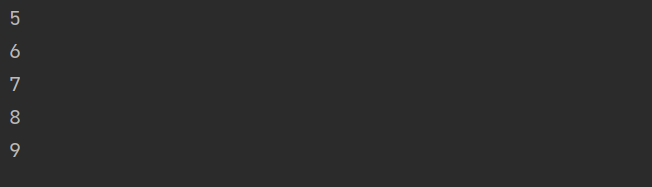
\includegraphics[width=8cm]{1D_Array.png}}
        \caption{One Dimensional Array}
    \end{center}
\end{figure*}
% 
% Section 7.2
% 
\section{Two Dimensional Array}
Two dimensional arrays are like matrix table. But each and every
element or position is a variable.
% 
% Subsection 7.2.1
% 
\subsection{Syntax}
\begin{center}
    \tt{
        \textit{dataType[][] arrayName = new dataType[][];}
    }
\end{center}

% 
% Subsection 7.2.2
%
\subsection{Example}
\begin{center}
    \footnotesize
    \begin{verbatim}
      import java.util.Scanner;
      public class Test {
          public static void main(String args[]) {
              Scanner input = new Scanner(System.in);
              System.out.print("Enter the row Number : ");
              int m = input.nextInt();
              System.out.print("Enter the Column Number : ");
              int n = input.nextInt();
              System.out.println("Enter Values : ");
              int [][] numbers = new int[m][n];
              for(int row=0;row<m;row++){
                  for(int col=0;col<n;col++){
                      System.out.print("Number["+(row+1)+"]["+(col+1)+"] = ");
                      numbers[row][col] = input.nextInt();
                  }
              }

              System.out.println("\n\nInsterd Values are =====>>");
              for(int row=0;row<m;row++){
                  for(int col=0;col<n;col++){
                      System.out.println("Number["+(row+1)+"]["+(col+1)+"] = "+numbers[row][col]);
                  }
              }
          }
      }
    \end{verbatim}
\end{center}
% 
% Figure 23 : Temp
% 
\begin{figure}[htbp]
    \begin{center}
        \fbox{\includegraphics*[width=8cm]{2D array.png}}
        \caption{temp\cite{Ref3}}
    \end{center}
\end{figure}
% 
% Section 7.3
% 
\section{ArrayList}
In short, arrayList is a dynamic array, where you can get as much as variables \\
but no overflow or null/underflow. As an example, suppose we need 5 variables \\
to store the marks of 5 students. but suddenly 3 students appears now if we use \\
normal array, then the storage is fixed with length 5 which means we have start \\
from the beginning again.But, if we use the arrayList, then we can add those 3 \\
students also without writing the code/software again. That's why it is also \\
called the better version of arrays. \linebreak
To add values in arrayList we need to use \textit{arrayListName.add(value);}
% 
% figure : 24
% 
\begin{table}[htbp]
    \begin{tabular}{|l|l|}
        \hline
        Array             & ArrayList              \\ \hline
        Not Resizable     & Resizable              \\ \hline
        For/For Each Loop & For Each Loop/Iterator \\ \hline
        Fast              & Slow                   \\ \hline
        arrayName.length; & arrayName.size();      \\ \hline
        Static            & Dynamic                \\ \hline
    \end{tabular}
    \centering
    \caption{Array VS ArrayList}
\end{table}
% 
% Subsection 7.3.1
% 
\subsection{Syntax}
\begin{center}
    \tt{
        \textit{ArrayList<dataType>variableName = new ArrayList();}
    }
\end{center}
% 
% Subsection 7.3.2
%
\subsection{Example}
\begin{center}
    \begin{verbatim}
        import java.util.ArrayList;
        import java.util.Scanner;

        import javax.print.attribute.standard.NumberUp;
        public class Test {
            public static void main(String args[]) {
                Scanner input = new Scanner(System.in);
                ArrayList<Integer>number = new ArrayList<>();
                System.out.println("Size = "+number.size());
                number.add(10);
                number.add(20);
                number.add(30);
                number.add(40);
                System.out.println(number); // Horizontal Print
                //using for each loop
                for(int x: number){
                    System.out.println(x);
                }
                System.out.println("Size = "+number.size());
                // Removing Elements
                number.remove(2);
                System.out.println("After Removing, Number = "+number);
                // REmoving all elements
                number.removeAll(number);
                System.out.println("After Removing All, Number = "+number);
                // Removing all Elements
                number.clear();
                System.out.println("After Removing, Number = "+number);
                boolean b = number.isEmpty();// Return true if empty
                System.out.println("Empty? = "+b);
                // Contaisn checks if the element is present or not
                boolean b1 = number.contains(30);
                System.out.println("Element Present ? = "+b1);
                // Index of shows index of any value, if not found then gives -1
                int i = number.indexOf(40);
                System.out.println("Index of the element = "+i);                
            }
        }
    \end{verbatim}
\end{center}
% 
% figure : 25 : 
% 
\begin{figure}[htbp]
    \begin{center}
        \fbox{\includegraphics*[width=8cm]{arrayList.png}}
        \caption{ArrayList\cite{Ref3}}
    \end{center}
\end{figure}
% 
% Subsection 7.3.3
% 
\subsection{Set Methods}
.set methods is used to replace any existing value present in any index of \\
arrayList. That means if we want to change the value of 5th index then the \\
arrayList should have the values from index 0 $\to$ 5.
% 
% Subsubsection 7.3.3.1
% 
\subsubsection{Syntax}
\begin{center}
    \tt{
        \textit{arrayListName.set(index,value);}
    }
\end{center}
% 
% Subsection 7.3.4
% 
\subsection{Get Methods}
.get methods is used to print any value present in any index of
arrayList.
% 
% Subsubsection 7.3.3.1
% 
\subsubsection{Syntax}
\begin{center}
    \tt{
        \textit{dataType variableName = arrayListName.get(indexNumber);}
    }
\end{center}
% 
% Subsubsection 7.3.3.2
%
\subsection{Example}
\begin{center}
    \begin{verbatim}
        import java.util.ArrayList;
        import java.util.Scanner;

        import javax.print.attribute.standard.NumberUp;
        public class Test {
            public static void main(String args[]) {
                Scanner input = new Scanner(System.in);
                ArrayList<Integer>number = new ArrayList<>();
                System.out.println("Size = "+number.size());
                number.add(10);
                number.add(20);
                number.add(30);
                number.add(40);
                System.out.println(number); // Horizontal Print
                //using for each loop
                for(int x: number){
                    System.out.println(x);
                }
                System.out.println("Size = "+number.size());
                // Removing Elements
                number.set(3,50);
                System.out.println("After Removing, Number = "+number);
                // REmoving all elements
                int x = number.get(3);
                System.out.println("Getting Value is = "+x); 
            }
        }
    \end{verbatim}
\end{center}
% 
% Figure 26 : ArrayList Set Get
% 
\begin{figure}[htbp]
    \begin{center}
        \fbox{\includegraphics*[width=8cm]{arrayListSETGET.png}}
        \caption{ArrayList Set Get\cite{Ref3}}
    \end{center}
\end{figure}
\subsection{ArrayList Methods}
\begin{table}[htbp]
    \begin{tabular}{ll}
        Method      & Task                                                                                       \\
        size()      & it shows the length/size                                                                   \\
        add()       & add value or element                                                                       \\
        remove()    & removes a specific element                                                                 \\
        removeAll() & removes every elements                                                                     \\
        clear()     & removes every elements                                                                     \\
        isEmpty()   & if yes, returns true                                                                       \\
        contains()  & \begin{tabular}[c]{@{}l@{}}if that specific element available,\\ return true\end{tabular}  \\
        indexOf()   & \begin{tabular}[c]{@{}l@{}}returns the index value if found,\\ else return -1\end{tabular} \\
        set()       & replace value of given index                                                               \\
        get()       & shows value of a specific index                                                            \\
        equal()     & shows if the arrayLists are equal or not                                                   \\
        addAll()    & Merge a arrayList into another
    \end{tabular}
    \centering
    \caption{ArrayList Methods}
\end{table}

\newpage

% 
% Subsection 7.3.4
% 
\subsection{Sorting ArrayList}
% 
% Subsubsection 7.3.4.1
% 
\subsubsection{Syntax}
\begin{center}
    \tt{
        \textit{Collections.sort(arrayListName);//Ascending\\Collections.sort(arrayListName,Collections.reverseOrder());//Reverse\\int variableName = ArrayListName.get(0);//Min\\int variableName = ArrayListName.size()-1);// Max}
    }
\end{center}
% 
% Subsubsection 7.3.4.1
% 
\subsubsection{Example}
\begin{center}
    \begin{verbatim}
        import java.util.ArrayList;
        import java.util.Collection;
        import java.util.Collections;
        import java.util.Scanner;

        import javax.print.attribute.standard.NumberUp;
        public class Test {
            public static void main(String args[]) {
                Scanner input = new Scanner(System.in);
                ArrayList<Integer>numbers = new ArrayList<>();//Declare ArrayList
                // Adding values to numbers
                numbers.add(50);
                numbers.add(30);
                numbers.add(10);
                System.out.println(numbers); 
                numbers.add(3,40); // Adding in a specific position
                System.out.println(numbers); 
                System.out.println("Size = "+numbers.size());
                // Ascending Sorting
                Collections.sort(numbers);
                System.out.println("After Ascending sorting = "+numbers);
                // Gettting Lowest value of ArrayList
                int min = numbers.get(0);
                System.out.println("Min Value = "+min);
                // Gettting Biggest value of ArrayList
                int max = numbers.get(numbers.size()-1);
                System.out.println("Max Value = "+max);
                // Descendind Sorting
                Collections.sort(numbers,Collections.reverseOrder());
                System.out.println("After Descending sorting = "+numbers);
            }
        }
    \end{verbatim}
\end{center}
% 
% Figure 27 : Temp
% 
\begin{figure}[htbp]
    \begin{center}
        \fbox{\includegraphics*[width=8cm]{Sorting ArrayList.png}}
        \caption{String Methods\cite{Ref3}}
    \end{center}
\end{figure}
% 
% Chapter 8
% 
\chapter{String}
Sequence of characters are together called strings. In simple words, words and \\
sentences are called strings.
% 
% Section : 8.1 
% 
\section{String Methods}
% 
% Subsection : 8.1.1
% 
\subsection{Syntax}
\begin{center}
    \tt{
        \textit{stringVariableName.methodName()}
    }
\end{center}
% 
% Subsection : 8.1.2
% 
\subsection{String Basic Methods}
% 
% Table 17
% 
\begin{table}[htbp]
    \begin{tabular}{ll}
        Method             & Description                                                                                               \\
        length()           & shows the string length                                                                                   \\
        equals()           & checks, 2 strings are same or not                                                                         \\
        equalsIgnoreCase() & \begin{tabular}[c]{@{}l@{}}matches the characters, doesn't matter\\ if it's capital or small\end{tabular} \\
        contains()         & checks if the word is present in the given string or not                                                  \\
        isEmpty()          & checks if the string is Empty {[}("") or null{]} or not                                                   \\
        concat()           & to add to strings together and make one string                                                            \\
        toUpperCase()      & It turns all the characters into upper case characters                                                    \\
        toLowerCase()      & It turns all the characters into lower case characters                                                    \\
        startsWith()       & It checks if the string started with given character or word                                              \\
        endsWith()         & It checks if the string ended with given character or word
    \end{tabular}
    \centering
    \caption{String Basic Methods}
\end{table}

\newpage

% 
% Subsection : 8.1.3
% 
\subsection{String Special Methods}
% 
% Table 18
% 
\begin{table}[htbp]
    \begin{tabular}{ll}
        Method        & TaskDescription                                                                                                                                             \\
        trim()        & Removes the previous after spaces in of a string                                                                                                            \\
        charAt()      & Takes an integer value as index \& return thing holding in that index variable                                                                              \\
        charPointAt() & Shows ASCII value based on input parameter                                                                                                                  \\
        indexOf       & Shows the index value of any character/word                                                                                                                 \\
        lastIndexOf() & \begin{tabular}[c]{@{}l@{}}If there is same character or word in a string then shows the index of the\\ last occurrence of that word/character\end{tabular} \\
        replace()     & It replaces all words that matches with the given word and puts new word                                                                                    \\
        split()       & It breaks when it founds the specific character and crops data till there
    \end{tabular}
    \centering
    \caption{String Special Methods}
\end{table}
% 
% Subsection : 8.1.4
% 
\subsection{Example}
\begin{center}
    \footnotesize
    \begin{verbatim}
        import java.util.ArrayList;
        import java.util.Collection;
        import java.util.Collections;
        import java.util.Scanner;

        import javax.print.attribute.standard.NumberUp;
        public class Test {
            public static void main(String args[]) {
                String message2 = "We_are_Learning";
                String message = "We_Are_Learning";
                System.out.println("Length = "+message.length());
                System.out.println("Equals = "+message.equals(message2));
                System.out.println("Equals Ingnoring Case = "+message.equalsIgnoreCase(message2));
                System.out.println("Contains = "+message.contains("Learning"));
                System.out.println("is Empty = "+message.isEmpty());
                System.out.println("Concat = "+message.concat("_Java"));
                System.out.println("To Upper Case = "+message.toUpperCase());
                System.out.println("To Lower Case = "+message.toLowerCase());
                System.out.println("Start With = "+message.startsWith("We"));
                System.out.println("Ends With = "+message.endsWith("Learning"));

                System.out.println("Trim = "+message.trim());
                System.out.println("Char At = "+message.charAt(5));
                System.out.println("Index Of = "+message.indexOf("Are"));
                System.out.println("Last index of = "+message.lastIndexOf("e"));
                System.out.println("Replace A -> a = "+message.replace('A','a'));
                String[] words = message.split("_");
                for (String string : words) {
                    System.out.println(string);
                }
            }
        }
    \end{verbatim}
\end{center}
% 
% Figure 28 : String Methods
% 
\begin{figure}[htbp]
    \begin{center}
        \fbox{\includegraphics*[width=8cm]{String Methods.png}}
        \caption{String Methods\cite{Ref3}}
    \end{center}
\end{figure}

\newpage

% 
% Section 8.2
% 
\section{String Buffer}
The only difference between string and string Buffer is, for string we can not \\
change the string and store at the same variable. Because we just make \\
association by just declaring string variables. But if we initialize string \\
object that means this is only operated inside that class no where else so \\
that's why we can change the string and store in that same variable.
% 
% table : 19
% 
\begin{table}[htbp]
    \begin{tabular}{ll}
        Method               & TaskDescription                                                                                                                                     \\
        append()             & Add a string with the existing string                                                                                                               \\
        reverse()            & \begin{tabular}[c]{@{}l@{}}It returns that same string but printed backwardly \\ as like (learn =$>$  nrael) \\ Also called Palindrome\end{tabular} \\
        delete(start,end)    & \begin{tabular}[c]{@{}l@{}}It deletes a specific portion of a string based on the\\ indexes\end{tabular}                                            \\
        setLength(parameter) & It show the strings from starting index 0 to parameter(integer)
    \end{tabular}
    \centering
    \caption{String Buffer Methods}
\end{table}
% 
% Subsection : 8.2.1
% 
\subsection{Syntax}
\begin{center}
    \tt{
        \textit{StringBuffer variableName = new StringBuffer(stringVariableName);\\variableName.methodName();}
    }
\end{center}
% 
% Subsection : 8.2.2
% 
\subsection{Example}
\begin{center}
    \begin{verbatim}
        public class Test {
            public static void main(String args[]) {
                String s1 = "boys";
                StringBuffer sb = new StringBuffer(s1);
                System.out.println(sb);
                sb.append(" are learning");
                sb.append(25);
                System.out.println(sb);
                sb.delete(0, 5);
                System.out.println(sb);
                sb.replace(0, 3, "We");
                System.out.println(sb);
                sb.reverse();
                System.out.println(sb);
            }
        }
    \end{verbatim}
\end{center}
% 
% Figure 29 : String Buffer Methods
% 
\begin{figure}[htbp]
    \begin{center}
        \fbox{\includegraphics*[width=8cm]{StringBuffer.png}}
        \caption{String Buffer}
    \end{center}
\end{figure}
% 
% Section 8.3
% 
\section{String Builder}
We can store string in 3 ways, those are,
\begin{itemize}
    \item String
    \item StringBuffer
    \item StringBuilder
\end{itemize}
Of them, StringBuffer and StringBuilder are similar.
% 
% Subsection 8.3.1
% 
\subsection{Syntax}
\begin{center}
    \tt{
        \textit{StringBuilder variableName = new StringBuider(stringVariableName);\\variableName.methodName();}
    }
\end{center}
% 
% Subsection 8.3.2
% 
\begin{center}
    \begin{verbatim}
        public class Test {
            public static void main(String args[]) {
            String s1 = "boys";
            StringBuilder message = new StringBuilder("We");
            System.out.println("String = "+message);
            message.append(" are learning");
            System.out.println("String updated = "+message);
            message.delete(2, 6);
            System.out.println(message);
        }
    }
    \end{verbatim}
\end{center}
% 
% Figure 30 : String Builder
% 
\begin{figure}[htbp]
    \begin{center}
        \fbox{\includegraphics*[width=8cm]{StringBuilder.png}}
        \caption{String Builder}
    \end{center}
\end{figure}
% 
% Chapter 9
% 
\chapter{Wrapper Class}
We know, int, charAt, double, these are primitive dataTypes. So, if we want to \\
convent these into a object or we want to convert an object Introduction \\
primitive dataTypes, then we'll need wrapper classes.
% 
% Table : 20
% 
\begin{table}[htbp]
    \begin{tabular}{cc}
        Primitive & Wrapper Class \\
        boolean   & Boolean       \\
        char      & Character     \\
        byte      & Byte          \\
        short     & Short         \\
        int       & Integer       \\
        long      & Long          \\
        float     & Float         \\
        double    & Double
    \end{tabular}
    \centering
    \caption{Wrapper Classes}
\end{table}
% 
% Subsubsection 9.0.0.1
% 
\subsubsection{AutoBoxing}
AutoBoxing means to convert a primitive dataType to an object.
% 
% Subsubsection 9.0.0.2
% 
\subsubsection{UnBoxing}
AutoBoxing means to convert an object to a primitive dataType.
% 
% Subsubsection 9.0.0.3
% 
\subsubsection{Syntax}
\begin{center}
    \tt{
        \raggedright{Auto Boxing Process-1 : \\}
        \textit{
            dataType variableName = value;\\
            wrapperClassType wrapperVariableName = wrapperClassType.valueOf(variableName);\\
        }
        \newpage
        \raggedright{Auto Boxing Process-2 : \\}
        \textit{
            dataType variableName = value;\\
            wrapperClassType wrapperVariableName = variableName;\\
        }
        \vskip 0.5cm
        \raggedright{Un-Boxing Process-1 : \\}
        \textit{
            wrapperClassType wrapperVariableName = new wrapperClassType(value);
            dataType variableName = wrapperVariableName.variableNameValue();
        }
        \vskip 0.5cm
        \raggedright{Un-Boxing Process-2 : \\}
        \textit{
            wrapperClassType wrapperVariableName = new wrapperClassType(value);\\
            dataType variableName = wrapperVariableName;\\
        }
    }
\end{center}
% 
% Subsubsection 9.0.0.4
% 
\subsubsection{Example}
\begin{center}
    \begin{verbatim}
        public class Test {
            public static void main(String args[]) {
                int x = 30;
                Integer z = x; // Auto-Boxing
                System.out.println("Z = "+z);
                Double d = new Double(10.25);
                System.out.println("d = "+d);
                double e = d; // UnBoxing
                System.out.println("e = "+e);
            }
        }
    \end{verbatim}
\end{center}
% 
% Figure 31 : AutoBoxing Unboxing
% 
\begin{figure}[htbp]
    \begin{center}
        \fbox{\includegraphics*[width=8cm]{BoxingUnBoxing.png}}
        \caption{AutoBoxing Unboxing}
    \end{center}
\end{figure}
% 
% Section 9.1
% 
\section{Conversation between String \& Primitive}
% 
% Subsection 9.1.1
% 
\subsection{Example}
\begin{center}
    \begin{verbatim}
        public class Test {
            public static void main(String args[]) {
            int i = 30;
            String s1 = Integer.toString(i); // int --> String
            System.out.println("S1 = "+s1);

            double d = 30.45;
            String s2 = Double.toString(d); // double --> String
            System.out.println("S2 = "+s2);
            
            String s3 = "32";
            int i2 = Integer.parseInt(s3); // String --> int
            System.out.println("i2 = "+i2);
            int ix = Integer.valueOf("100");
            System.out.println("ix = "+i);
        }
    }
    \end{verbatim}
\end{center}
% 
% Figure 32 : String & Primitive
% 
\begin{figure}[htbp]
    \begin{center}
        \fbox{\includegraphics*[width=8cm]{StringAndPrimitive.png}}
        \caption{String \& Primitive}
    \end{center}
\end{figure}
% ************* Code********
\begin{center}
    \begin{verbatim}
        public class Test {
            public static void main(String args[]) {
            int decimal = 15;
            String binary = Integer.toBinaryString(decimal);//decimal --> Binary
            System.out.println("Binary = "+binary);

            String octal = Integer.toOctalString(decimal); // decimal --> Octal
            System.out.println("Octal = "+octal);

            String hexa = Integer.toOctalString(decimal); // decimal --> Octal
            System.out.println("Hexa = "+hexa);
        }
    }
    \end{verbatim}
\end{center}
% 
% Figure 33 : Decimal --> Binary/Octal/Hexa-Decimal
% 
\begin{figure}[htbp]
    \begin{center}
        \fbox{\includegraphics*[width=8cm]{DecimalToBinOctHexa.png}}
        \caption{Decimal $-->$ Binary/Octal/Hexa-Decimal}
    \end{center}
\end{figure}
% ************* Code********
\begin{center}
    \begin{verbatim}
        public class Test {
            public static void main(String args[]) {
                String binary = "101101";
                int decimal = Integer.parseInt(binary,2); // binary --> Decimal
                System.out.println("Decimal = "+decimal);
        
                String octal = "675";
                int decimal_2 = Integer.parseInt(octal,8); // octal --> Decimal
                System.out.println("Decimal_2 = "+decimal_2);
        
                String hexa = "70AF";
                int decimal_3 = Integer.parseInt(hexa,16); // hexa --> Decimal
                System.out.println("Decimal_3 = "+decimal_3);
        }
    }
    \end{verbatim}
\end{center}
% 
% Figure 33 : Binary/Octal/Hexa-Decimal --> Decimal
% 
\begin{figure}[htbp]
    \begin{center}
        \fbox{\includegraphics*[width=8cm]{BinOctHexaToDecimal.png}}
        \caption{Binary/Octal/Hexa-Decimal $-->$ Decimal}
    \end{center}
\end{figure}
% 
% Section 9.2
% 
\section{Date Class}
This `Date' class is the only class which we can use to see the normal date by \\
formatting.
% 
% Subsection 9.2.1
% 
\subsection{Syntax}
\begin{center}
    \tt{
        \raggedright{System-1 :}\\
        \textit{
            Date date = new Date();\\
        }
        \vskip 0.5cm
        \raggedright{System-2 :}\\
        \textit{
            Date date = new Date();\\
            DateFormat dateFormat = new SimpleDateFormat("dd/MM/YYYY");\\
            String currentDate = dateFormat.format(date);\\
        }
    }
\end{center}

\newpage

% 
% Subsection 9.2.2
% 
\subsection{Example}
\begin{center}
    \begin{verbatim}
        import java.text.DateFormat;
        import java.text.SimpleDateFormat;
        import java.util.Date;

        public class Test {
            public static void main(String args[]) {
                Date date = new Date();
            System.out.println("Date Class = "+date);

            // Formatting Time (My choice)
            DateFormat dateFormat = new SimpleDateFormat("dd/MM/YYYY");
            String currentDate = dateFormat.format(date);
            System.out.println("Current Date(My choice format) : "+currentDate);
        }
    }
    \end{verbatim}
\end{center}
% 
% Figure 33 : Date Class
% 
\begin{figure}[htbp]
    \begin{center}
        \fbox{\includegraphics*[width=8cm]{DateClass.png}}
        \caption{Date Class}
    \end{center}
\end{figure}
% 
% Section 9.3
% 
\section{Time Class}
Time class is used to receive current time.
% 
% Subsection 9.3.1
% 
\subsection{Example}
\begin{center}
    \tt{
        \raggedright{System-1 :}\\
        \textit{
            LocalTime time = LocalTime.now();\\
        }
        \vskip 0.5cm
        \raggedright{System-2 :}\\
        \textit{
            LocalTime time = LocalTime.now();\\
            DateTimeFormatter formatter = DateTimeFormatter.ofPattern("hh:mm:ss");\\
            String currentTime = time.format(formatter);\\
        }
    }
\end{center}

\newpage

% 
% Subsection 9.3.2
% 
\subsection{Example}
\begin{center}
    \footnotesize
    \begin{verbatim}
        import java.time.LocalTime;
        import java.time.format.DateTimeFormatter;

        public class Test {
            public static void main(String args[]) {
                public static void main(String args[]) {
                LocalTime time = LocalTime.now();
                System.out.println("Time Class = "+time);

                // Formatting Time (My choice)
                DateTimeFormatter formatter = DateTimeFormatter.ofPattern("hh:mm:ss");
                String currentTime = time.format(formatter);
                System.out.println("Current Date(My choice format) : "+currentTime);
            }
        }
    \end{verbatim}
\end{center}
% 
% Figure 34 : Time Class
% 
\begin{figure}[htbp]
    \begin{center}
        \fbox{\includegraphics*[width=8cm]{TimeClass.png}}
        \caption{Time Class}
    \end{center}
\end{figure}
% 
% Section 9.4
% 
\section{Random Number}
Random number means the program will generate any digit or multi-digit number \\
automatically. We can do this by using,
\begin{itemize}
    \item Random Class
    \item Math Class
\end{itemize}
% 
% Subsubsection 9.4.0.1
% 
\subsubsection{Syntax}
\begin{center}
    \tt{
        \raggedright{By using Random Class : }\\
        \textit{
            Random rand = new Rand();\\
            System.out.println($rand.nextInt(rangeValueFrom_0)$);\\
        }
        \vskip 0.5cm
        \raggedright{By using Math Class : }\\
        \textit{
            System.out.println($Math.random()*rangeValueFrom_0$);\\
        }
    }
\end{center}

\newpage

% 
% Subsubsection 9.4.0.2
% 
\subsubsection{Example}
\begin{center}
    \footnotesize
    \begin{verbatim}
        import java.util.Random;
        public class Test {
            public static void main(String args[]) {
                // By using Random Class
                Random rand = new Random();
                int randomNumber = rand. nextInt(10);// from 0 --> 10
                System.out.println("Random Value 1 = "+randomNumber+50);
                int randomNumber1 = rand. nextInt(10)+50;
                System.out.println("Random Value 2 = "+randomNumber1); // from 50 --> (50+10 = 60)

                // By using Math Class
                int randomNumber2 = (int) (Math.random()*20); // from 0 --> 20
                System.out.println("Random Value 2 = "+randomNumber2); 
                int randomNumber3 = (int) (Math.random()*20)+30; // from 30 --> (30+20 = 50)
                System.out.println("Random Value 4 = "+randomNumber3); 
            }
        }
    \end{verbatim}
\end{center}
% 
% Figure 35 : Random Number
% 
\begin{figure}[htbp]
    \begin{center}
        \fbox{\includegraphics*[width=8cm]{Random.png}}
        \caption{Random Number}
    \end{center}
\end{figure}

% 
% Part 4 
% 
\part{Object Oriented Programming}
\vspace*{\fill}
As the name suggests, object-oriented programming or OOPs refers to languages
that use objects in programming, they use objects as a primary source to \\
implement what is to happen in the code. Objects are seen by the viewer or \\
user, performing tasks assigned by you.
\vspace*{\fill}

% 
% Chapter 10
% 
\chapter{Introduction to Object Oriented Programming}
In this chapter we'll learn about the basic things of OOP(Object Oriented \\
Programming). Mainly OOP is based on some core features. Those are,
\begin{itemize}
    \item Encapsulation
    \item Classes
    \item Inheritance
    \item Abstraction
    \item Polymorphism
    \item Access modifiers
    \item Interface
\end{itemize}
% 
% Figure 36 : OOP concept overview
% 
\begin{figure}[htbp]
    \begin{center}
        \fbox{\includegraphics*[width=8cm]{OOP.png}}
        \caption{OOP concept overview}
    \end{center}
\end{figure}

\newpage

% 
% Subsubsection 10.0.0.1
% 
\subsubsection{Object}
Everything we can see around us is called an object. More specifically, \\
Variables or instance of any class is called an object.
% 
% Subsubsection 10.0.0.2
% 
\subsubsection{Class}
Common collection of many objects is called a class. More specifically, class \\
is a thing which holds variables and methods inside it.
% 
% Section 10.1
% 
\section{Introducing Class}
A class in java is basically a template that we can use multiple times. There \\
are 3 major portion of a class. Those are,
\begin{itemize}
    \item Class Name
    \item Attributes/Variables
    \item Methods
\end{itemize}
% 
% Figure 37 : Class Structure
% 
\begin{figure}[htbp]
    \begin{center}
        \fbox{\includegraphics*[width=8cm]{ClassStructure.png}}
        \caption{Class Structure}
    \end{center}
\end{figure}
% 
% Subsection 10.1.1
% 
\subsection{Class Name}
Every class must have a class name. Class name has also a access modifier \\
public/private/default. If we use default or no access modifier, then it can \\
oly be accessed from that folder. So to use this globally we need to declare \\
it as public. And if we declare it as public, then we have to keep the \\
fileName.java as same as the className. \\
That means file name would be == className.java
% 
% Subsubsection 10.1.1.1
%
\subsubsection{Syntax}
\begin{center}
    \raggedright
    \tt{
        \textit{
            \quad\quad\quad\quad\quad\quad\quad\quad\quad\quad\quad\quad\quad public class className\{ \\
            \quad\quad\quad\quad\quad\quad\quad\quad\quad\quad\quad\quad\quad\quad\quad // Attributes \\
            \quad\quad\quad\quad\quad\quad\quad\quad\quad\quad\quad\quad\quad\quad\quad //Methods \\
            \quad\quad\quad\quad\quad\quad\quad\quad\quad\quad\quad\quad\quad \}
        }
    }
\end{center}
% 
% Subsection 10.1.2
% 
\subsection{Attributes/Variables}
After declaring the class name. Now heading part of any class is basically \\
attributes or in other words, you can say here we normally declare all our \\
variables and objects classes that is going to be used in the whole class.
% 
% Subsection 10.1.3
% 
\subsection{Methods}
After declaring all the variables, that we need initially, then we'll go for \\
methods. What is called methods we will learn next.
% 
% Section 10.2
%
\section{Object Declaration \& Creation}
Object of a class means creating an instance of that class. That means all the \\
things of that class which is public, we can access them by using that instance \\
or object.
























% 
% INDEX
% 
\printindex
% 
% BIBLIOGRAPHY
% 
\begin{thebibliography}{90}
    \footnotesize
    \bibitem{Ref1} Java, \url{en.wikipedia.org/wiki/Java_(programming_language)}
    \bibitem{Ref2} James Gosling, \url{en.wikipedia.org/wiki/James_Gosling}
    \bibitem{Ref3} Java Compiler, \url{www.jdoodle.com/online-java-compiler/}
    \bibitem{Ref4} Escape Sequence, \url{docs.oracle.com/javase/tutorial/java/data/characters.html}
    \bibitem{Ref5} Format Specifier,  \footnotesize{\url{www.geeksforgeeks.org/format-specifiers-in-java/}}
    \bibitem{Ref6} DataType, \url{www.javatpoint.com/java-data-types}
    \bibitem{Ref7} User Input, \url{www.w3schools.com/java/java_user_input.asp}
    \bibitem{Ref8} Operators, \url{www.qafox.com/java-for-testers-different-types-of-operators-in-java/}
    \bibitem{Ref9} Control Statements, \\ \raggedright{\url{www.testingtools.co/java/11-keywords-to-learn-loops-and-conditional-statements-in-java}}
    \bibitem{Ref10} Vending Machine, \url{www.benchmarkreporter.com/buying-vs-renting-a-vending-machine-which-option-is-better/}
\end{thebibliography}



















%%%%%%%%%%%%%%%%%%%%%%%%%%%%%%%%%%%%%%%%%%%%%%%%%%%%%%%%%%%%%%%%%%%%%%%%%%%%%%%%%%%%%%%%%%%%%%%%%%%%%%%%%%%%%%%%%%%%%%%%%%%%%%%%%%%%%%%%%%%%%%%%%%%%%%%%%%%%%%%%%%%%%%%%%%%%%%%%%%%%%%%%%%%%%%%%%%%%
%%%%%%%%%%%%%%%%%%%%%%%%%%%%%%%%%%%%%%%%%%%%%%%%%%%%%%%%%%%%%%%%%%%%%%%%%%%%%%%%%%%%%%%%%%%%%%%%%%%%%%%%%%%%%%%%%%%%%%%%%%%%%%%%%%%%%%%%%%%%%%%%%%%%%%%%%%%%%%%%%%%%%%%%%%%%%%%%%%%%%%%%%%%%%%%%%%%%



\vspace*{\fill}
\end{document}

% \index{Index B}
% \chapter{Chapter 2 of Part 2}
% \index{Index C}
% \addtocontents{toc}{DESCRIPTION} % Used for writing a DESCRIPTION of any chapter/section, It means the name will added in contents but page no does not appear
% \section{Section of Chapter 2 of part 2}

% 
% Figure 0 : Temp
% 
\begin{figure}[htbp]
    \begin{center}
        \fbox{\includegraphics*[width=8cm]{temp.png}}
        \caption{temp\cite{Ref3}}
    \end{center}
\end{figure}

% 
% Part 1
% 
\index{Private}

\cite{Ref1}

% 
% Subsection 3.2.1
%
\subsection{Syntax}
\begin{center}
    \tt{
        \textit{"\%formatSpecifier"}
    }
\end{center}

% 
% Subsection 3.2.2
%
\subsection{Example}
\begin{center}
    \begin{verbatim}
        ...
    \end{verbatim}
\end{center}



\the \evensidemargin\\
\the \oddsidemargin

\vskip 0.5cm

% ************* Code********
\begin{center}
    \begin{verbatim}
        public class Test {
            public static void main(String args[]) {
                
        }
    }
    \end{verbatim}
\end{center}


\vspace*{\fill}
This text will be centered vertically
\vspace*{\fill}